In this section we include the average shape measurement 
bias results on a representative DES lensing catalog of 
all sources SNR $>$ 20. Most previous weak lensing studies 
rejected all objects below a set SNR threshold, but the 
depth chosen varies as it is determined by both the capabilities 
of the lensing pipeline used and the type of lensing analysis sought. In 
the CFHTLens survey all objects were rejected that were
measured as i'(AB) $<$ 24.7, or a SNR limit of around 10
\citep{cfhtls}. This limit was imposed for the CFHTLenS
catalog as it was the depth determined at which the 
photometric redshifts and shape measurements were too
poorly measured \citep{Hild}. For the CSTEP project
we chose objects SNR $>$ 20 for the representative DES 
lensing catalog. This is a conservative choice, and 
with additional lensing pipeline development a lower
SNR threshold could be chosen for the final DES 
lensing catalog. \\
\indent The average shape measurement bias on all images 
in the CSTEP simulations for galaxies SNR $>$ 20
is shown in Figure \ref{fig:QMC}. 
\begin{figure}
 \centering  % this centres figure in column
  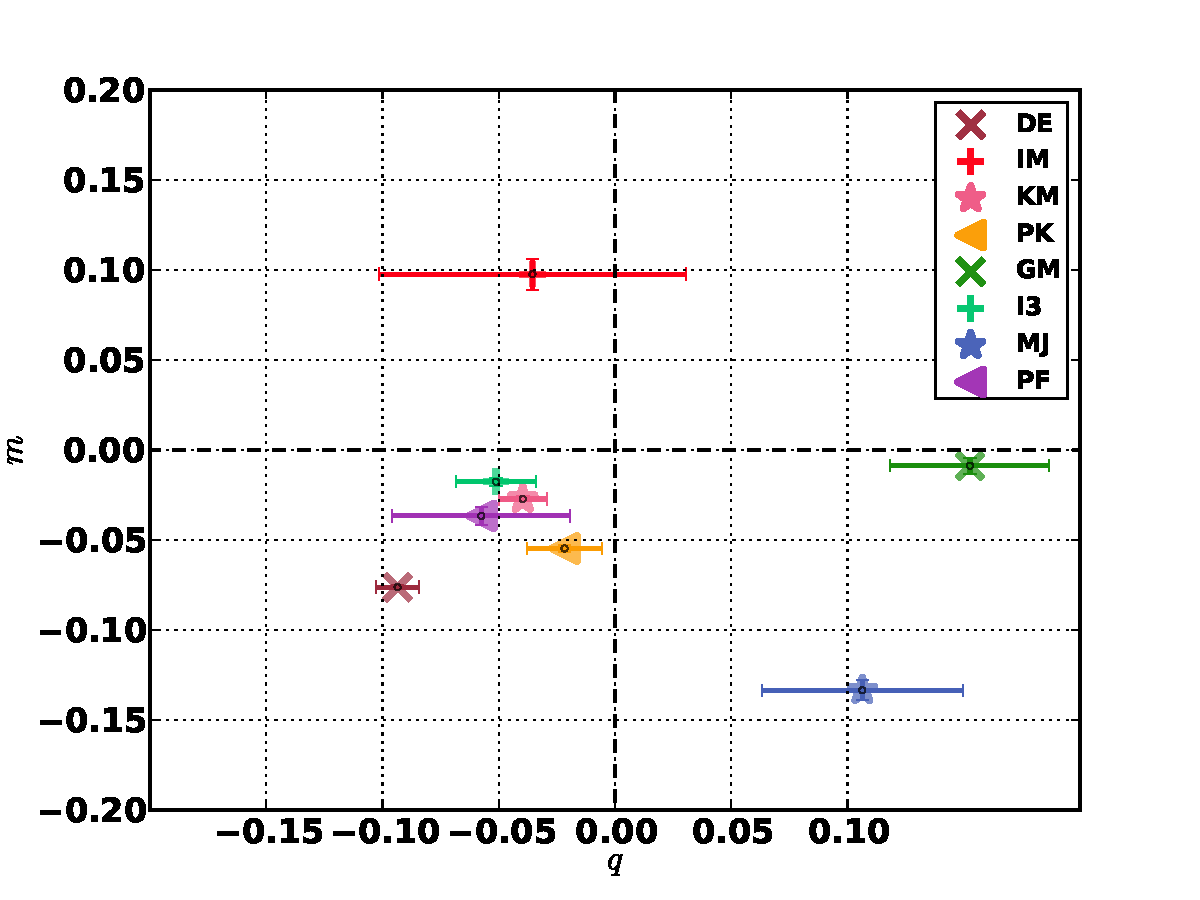
\includegraphics[width=0.45\textwidth]{fig/QMC_main_f.pdf} 
  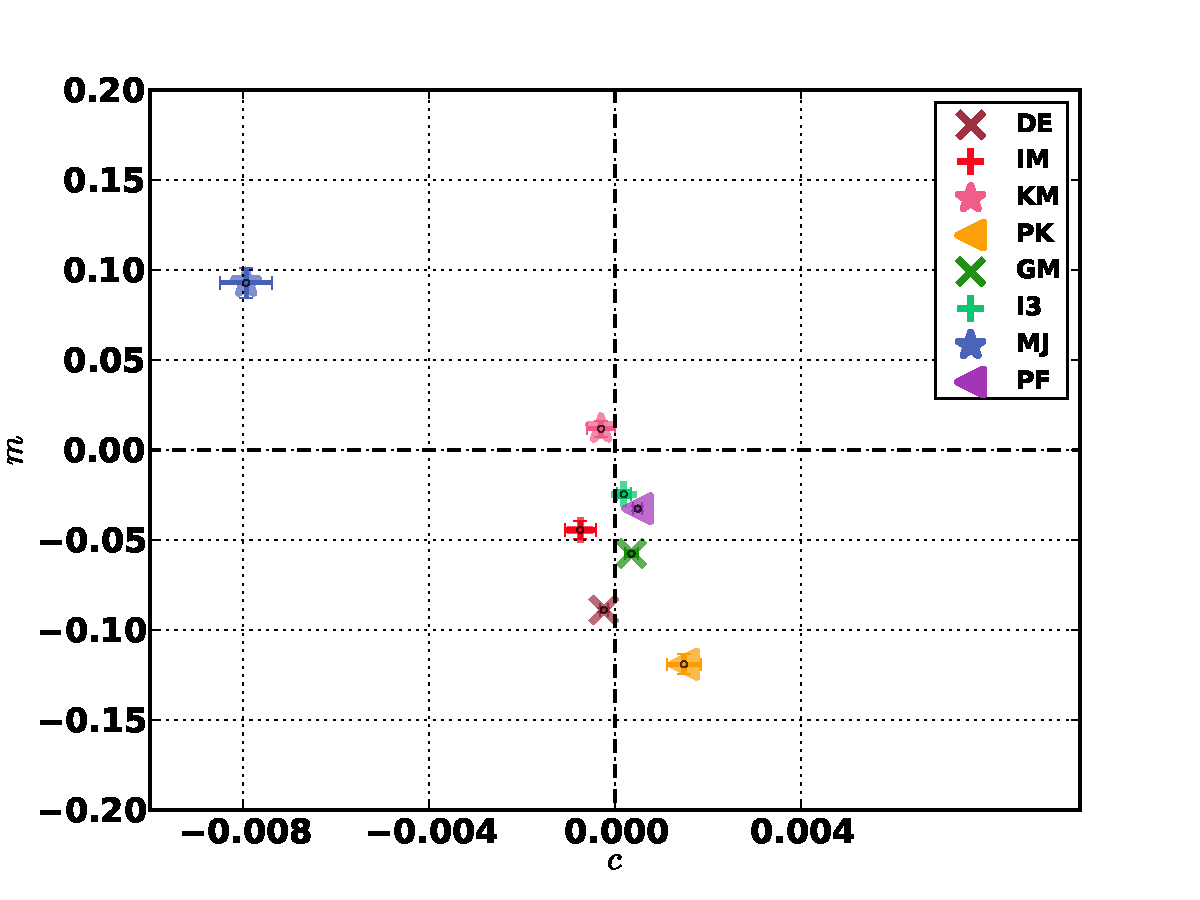
\includegraphics[width=0.45\textwidth]{fig/MC_main_f.pdf} 
  \caption{This figure shows the average shape measurement bias
as measured on all images for galaxy objects SNR $>$ 20. The
top panel shows the shape measurement bias $q$,$m$ as measured using 
a $q$,$m$,$c$ fit. The bottom panel shows the shape measurement bias 
$m$,$c$ as measured using a $m$,$c$ fit.}
\label{fig:QMC}
\end{figure}
Three of the lensing pipelines (I3, DE, KM) that are included in the
cluster STEP results, also competed in the GREAT10 challenge.
%The comparison between the GREAT10 and CSTEP results is shown in 
%Figure \ref{fig:gt10}. 
The results are roughly consistent between
the two challenges for I3 and KM showing that both pipelines are 
robust, and demonstrate similar levels of shape measurement bias
for a wide variety of sources and PSF types. Both I3 and KM are 
among the best performing lensing pipelines for both CSTEP and
GREAT10. 

